% =================================================
% SHEEPLE TO DO BOARD AND NOTES
% =================================================
% Fill in unfilled sections
%
% If there is great blank space, we can merge
% some of them. Currently, I believe there is not
% going to be enough sections dedicated to Scalettar.
%
% Update components and materials table to make it accurate.
%
% Can one of you guys send an image of the output of the STM
% machine into the group chat? I need to make a code to convert
% the thing into images on matplotlib.
%
% DATA OUTPUT AND SURFACE RECONSTRUCTION:
% - Once we get a complete scan, add the forward, backward, and
%   parameter files here.
% - Finish the Python code that reads everything and turns it into
%   the scan matrix.
% - Double-check which way x and y go, then compare the forward and
%   backward scans to see if anything drifted or got offset.
% - Figure out the z-piezo calibration before calling anything an
%   actual height.
% - Make the final Matplotlib 2D map and maybe a 3D version too.
% - Put the raw data, working code, settings, and final figures in
%   clustered when we have them.
%
%
% =================================================
% FORMATTING CONVENTIONS
% =================================================
% - A section is a different main category. If two sections share one sheet,
%   put \categorygap between them so the gap is always 2 cm.
% - Subsections and subsubsections are parts of the same category. LaTeX gives
%   them a 1 cm gap automatically, so do not add random \vspace commands.
% - The first paragraph after a heading stays unindented. Later paragraphs in
%   the same block use the normal 1.5 em indent.
% - Normal body text uses 1.12 line spacing. The three crowded software or
%   formula sheets can use 1.0 spacing inside their existing spacing blocks.
% - Keep figures centered with the caption right below. Put the citation in the
%   caption too if the picture or diagram came from one of our sources.
% - Keep everything black and white except real Matplotlib data graphs.
% - Use booktabs-style tables: no vertical lines, units in the labels, and no
%   made-up values in blank result tables.
% - Every printed sheet ends with \clearpage. Do not use manual line breaks to
%   force a page layout when a proper paragraph or spacing command works.
% - Keep main.tex and every PNG it uses directly inside transform so we can
%   upload the whole folder to Overleaf at once.
%
% =================================================
% POSTER LAYOUT MAP
% =================================================
% TOP
%   Title block will be created separately in Overleaf
%
% LEFT PANEL
%   1. Abstract + Introduction and Motivation
%      + Data Provenance and Visualization Notice
%   2. Theoretical and Technical Background
%   3. Instrument Design and Construction
%
% CENTER PANEL
%   The top-center row remains empty in the assembled poster.
%
%   HARDWARE COLUMN             SOFTWARE COLUMN
%   4. Hardware Architecture    5. Control Software Architecture
%   6. Operating Principles     7. Control Logic and Scan Execution
%   8. Testing and Calibration  9. Data Output and Surface Reconstruction
%
% RIGHT PANEL
%   10. Results and Uncertainty Analysis
%   11. Supplementary Figures
%   12. References and Acknowledgments, with GitHub QR code at top right

\documentclass[9pt,oneside]{report}

% =================================================
% PACKAGES
% =================================================
\usepackage[letterpaper,margin=1in]{geometry}
\usepackage{graphicx}
\usepackage{amsmath}
\usepackage{amssymb}
\usepackage{booktabs}
\usepackage{float}
\usepackage{array}
\usepackage{setspace}
\usepackage{caption}
\usepackage{titlesec}
\usepackage{listings}
\usepackage{microtype}
\usepackage{newtxtext}
\usepackage{newtxmath}
\usepackage{pdflscape}
\usepackage[hidelinks]{hyperref}
\usepackage{qrcode}

% =================================================
% COLOR AND TYPOGRAPHY
% =================================================
\setstretch{1.12}
\setlength{\parindent}{1.5em}
\setlength{\parskip}{0pt}
\setlength{\emergencystretch}{3em}
\raggedbottom
\renewcommand{\arraystretch}{1.12}

% Use this only between two completely different sections on the same sheet.
% Subsection spacing is already handled below.
\newcommand{\categorygap}{\par\vspace{2cm}}

\setcounter{secnumdepth}{0}

\titleformat{\section}
  {\normalfont\Large\bfseries\centering}
  {}
  {0pt}
  {\MakeUppercase}

\titleformat{\subsection}
  {\normalfont\large\bfseries}
  {}
  {0pt}
  {}

\titleformat{\subsubsection}
  {\normalfont\normalsize\bfseries}
  {}
  {0pt}
  {}

\titlespacing*{\section}{0pt}{0pt}{14pt}
\titlespacing*{\subsection}{0pt}{1cm}{4pt}
\titlespacing*{\subsubsection}{0pt}{1cm}{3pt}

\captionsetup{
  font=small,
  labelfont=bf,
  justification=centering,
  skip=5pt
}

\lstset{
  language=C++,
  basicstyle=\ttfamily\scriptsize,
  frame=single,
  breaklines=true,
  columns=fullflexible,
  keepspaces=true,
  showstringspaces=false,
  aboveskip=4pt,
  belowskip=4pt
}

\pagestyle{empty}
\urlstyle{same}

% =================================================
% DOCUMENT
% =================================================
\begin{document}

% =================================================
% LEFT PANEL: THREE PORTRAIT SHEETS
% =================================================

% -------------------------------------------------
% SHEET 1 OF 12 -- ABSTRACT + INTRODUCTION/MOTIVATION
%                 + DATA PROVENANCE/VISUALIZATION NOTICE
% -------------------------------------------------
% These three sections are sharing one sheet on purpose. Keep the 2 cm gaps
% below so they still look like separate parts when we print everything.
\section{Abstract}

% Keep this as the short version of the whole project. Once the STM is fully
% tested, update the last paragraph with what it actually did.
This project aims to design, construct, and test a scanning tunneling
microscope (STM) capable of measuring the surface topography of a conductive
sample at the nanoscale. An STM operates by applying a voltage bias between a
sharp metallic tip and the sample. When the tip is brought within a few
angstroms of the surface, electrons quantum mechanically tunnel across the
gap, producing a current that varies exponentially with tip--sample distance.

The instrument combines a piezoelectric scanner, coarse-positioning stepper
motor, current preamplifier, analog-to-digital converter, dual-rail power
supply, and vibration-isolation system. The tunneling-current signal is
measured and used by a feedback system to adjust the vertical position of the
tip. By maintaining a nearly constant current while scanning laterally, the
system can relate the required tip motion to changes in surface height.

Subsystem testing confirmed the operation of the power supply, preamplifier,
and analog-to-digital conversion stages. The final performance of the STM is
limited by mechanical vibration, electrical noise, thermal drift, tip
sharpness, and calibration accuracy. These tests establish the operating
principles of the instrument and identify the improvements needed to achieve
stable, repeatable nanoscale imaging.

\categorygap

\section{Introduction and Motivation}

% This part is more about why we made an STM, so do not repeat all the hardware
% details from the abstract here.
Scanning tunneling microscopy connects quantum mechanics to a practical
measurement technique. Because tunneling current is highly sensitive to
tip--sample separation, a feedback-controlled STM can detect very small
variations across a conductive surface. This project also integrates several
areas studied during COSMOS: wavefunctions and Hamiltonians, precision
current measurement, ADC and DAC conversion, PID feedback, piezoelectric
positioning, vibration isolation, and computational data collection.
Constructing an STM therefore provided both a nanoscale surface-measurement
goal and a practical demonstration of how quantum physics, electronics,
programming, and mechanical design operate
together.\textsuperscript{[1--3]}

\categorygap

\section{Data Provenance and Visualization Notice}

% Keep this notice even after the conversion code works. It makes it clear that
% the final map is processed data and not a photograph from the microscope.
% Insert the exact raw-data and code paths here for future once they are in
% clustered.
The values recorded by the STM are the instrument's original measurement
output. Any surface image or three-dimensional rendering shown later is a
processed visualization produced by passing those measurements through a
separate modeling program; it is not a direct photograph from the STM. The
original STM data, the processed output, and the code used to convert the
measurements into a model will be added to the
\href{https://github.com/souuk/clustered}{clustered GitHub repository} as they
become available.

\clearpage

% -------------------------------------------------
% SHEET 2 OF 12 -- THEORETICAL AND TECHNICAL BACKGROUND
% -------------------------------------------------
\section{Theoretical and Technical Background}

% The spacing is tighter on this page because the formulas take up a lot of
% room. If this page ends up looking empty later, change 1.0 back to 1.12.
\begin{spacing}{1.0}
\setlength{\abovedisplayskip}{6pt}
\setlength{\belowdisplayskip}{6pt}

\subsection{Quantum-Mechanical Description}

% This is the quantum background from Chiang's notes. Keep the citation on both
% the explanation and the formula since both came from the notes.
Professor Chiang's notes describe an electron using a complex
wavefunction.\textsuperscript{[1]} For a model containing \(M\) possible
sites, the wavefunction is a vector with one component for each site. The
squared magnitude of a component gives the probability of finding the
electron at that location.\textsuperscript{[1]} A Hamiltonian matrix describes
the system's energy, and its eigenvalues and eigenvectors determine how the
state changes with time.\textsuperscript{[1]}
\[
  P(j)=\lvert\psi_j\rvert^2,
  \qquad
  \psi(t)=e^{-iHt}\psi(0).
  \tag*{\text{\textsuperscript{[1]}}}
\]
This framework connects quantum probability to the vectors, matrices, and
time-evolution calculations studied in computational
physics.\textsuperscript{[1]}

\subsection{STM Signal Measurement}

% This is where the tiny current becomes a number the Teensy can actually use.
% If we measure a different resistor or ADC range later, update both the text
% and the formula together.
The supplied STM system converts a very small tunneling current into digital
data.\textsuperscript{[2]} Its preamplifier uses a
\(500\,\mathrm{M}\Omega\) feedback resistor and produces \(-0.5\) V for a
current of \(1\) nA.\textsuperscript{[2]} An 18-bit ADS8691
analog-to-digital converter maps voltages from \(-12.288\) to \(+12.288\) V
into integer values from \(0\) to \(262143\), with zero volts at
\(N_0=131072\).\textsuperscript{[2]} The controller converts each ADC reading
\(N\) back into a voltage using
\[
  V_{\mathrm{ADC}}
  =\frac{(N-N_0)(12.288\ \mathrm{V})}{N_0}.
  \tag*{\text{\textsuperscript{[2]}}}
\]
The program also uses a four-channel 16-bit DAC to control the \(x\), \(y\),
and \(z\) piezo signals and the sample-bias voltage. Its default sample bias
is \(1.0\) V, represented by approximately \(2282\) DAC
counts.\textsuperscript{[2]}

\subsection{Approach, Feedback, and Topographic Mapping}

% This paragraph connects the physics to what the program actually does.
% Insert our final approach threshold and PID settings here for future if they
% end up being different from the supplied defaults.
During the automated approach, the program gradually extends the \(z\)-piezo
and repeatedly measures the current. A reading greater than \(0.2\) nA in
magnitude must be detected twice before the approach stops and feedback is
enabled.\textsuperscript{[2]} This repeated check helps prevent a single noisy
reading from being treated as a tunneling signal.\textsuperscript{[2]}

Once feedback is active, the included PID routine compares the measured ADC
value with the chosen current setpoint. It updates the \(z\)-piezo output
every \(100\,\mu\mathrm{s}\), using proportional, integral, and derivative
terms to reduce the error.\textsuperscript{[2,3]} During imaging, a second
timer records points while the DAC moves through the \(x\) and \(y\)
coordinates.\textsuperscript{[2]} The program stores forward and backward
scan lines separately so the two directions can be
compared.\textsuperscript{[2]}

\end{spacing}

\clearpage

% -------------------------------------------------
% SHEET 3 OF 12 -- INSTRUMENT DESIGN AND CONSTRUCTION
% -------------------------------------------------
\section{Instrument Design and Construction}

% Talk about what we physically built and how we put it together here.
% Save the testing stuff for Sheet 8.

\subsection{Components and Materials}

% This is only a selected list right now. Insert the full final parts list here
% for future once everyone agrees on what was actually used.
\begin{table}[H]
  \centering
  \small
  \begin{tabular}{>{\raggedright\arraybackslash}p{0.78\textwidth}r}
    \toprule
    Component & Quantity \\
    \midrule
    Positive and negative adjustable voltage regulators & 1 each \\
    \(2200\,\mu\mathrm{F}\), 35 V capacitors & 2 \\
    \(1\,\mu\mathrm{F}\), 35 V tantalum capacitors & 2 \\
    General-purpose rectifier diodes & 4 \\
    \(1\,\mathrm{k}\Omega\) and \(180\,\Omega\) resistors & 1 and 2 \\
    \(2.5\,\mathrm{k}\Omega\) trimmer potentiometers & 2 \\
    12.6 V center-tapped transformer & 1 \\
    TO-220 heat sinks & 2 \\
    Machine screws, lock washers, and hex nuts & As required \\
    \bottomrule
  \end{tabular}
  \caption{Selected power-supply and mechanical components.}
\end{table}

\subsubsection{Dual-Rail Power Supply}

% Insert a clear photo of the finished power-supply board here for future.
% Try to use one where the wiring and the +15 V / -15 V labels are readable.
The power supply provides stable \(+15\) V and \(-15\) V rails. It was
constructed from a provided circuit board, resistors, capacitors,
transformers, regulators, and related components. The components were
soldered to the board, installed in a 3D-printed enclosure, and checked with
a multimeter. Trimmer potentiometers were adjusted until both output rails
reached their target voltages relative to ground.

\subsubsection{Piezoelectric Scanner}

% Insert a labeled close-up of the piezo and tip here for future if we have one.
The piezoelectric scanner provides fine \(x\), \(y\), and \(z\) positioning
of the tip. A voltage bias between the metallic tip and conductive sample
allows a tunneling current to form when their separation becomes sufficiently
small. During scanning, the lateral piezo signals move the tip across the
sample while feedback controls its vertical position.

\subsubsection{Coarse-Approach Mechanism}

% Insert a photo showing the motor, plates, and direction of movement here for
% future. A side view would probably explain this better than a top view.
The stepper-motor mechanism provides coarse positioning so the tip can be
brought into the operating range of the piezoelectric scanner. The mechanism
was assembled from metal plates, screws, and a geared stepper motor. The
piezoelectric scanner was mounted at the center of the mechanism.

\subsubsection{Vibration-Isolation System}

% Insert a full photo of the suspended platform here for future. Label the
% springs, magnets, and added weights if the picture is not obvious by itself.
The spring-suspension system isolates the microscope from external
vibrations. Professor Shirley Chiang provided the suspended platform.
Magnetic stabilizers were added at the base and sides to damp motion, and
weights were added to bring the suspended platform into the effective range
of the magnets. The stepper-motor assembly was then placed on the platform.

\clearpage

% =================================================
% CENTER PANEL: SIX LANDSCAPE SHEETS
% =================================================
% In the assembled center panel, Sheets 4, 6, and 8 form the hardware column.
% Sheets 5, 7, and 9 form the software/computation column.
% The row above these six sheets is intentionally left empty.

\begin{landscape}

% -------------------------------------------------
% CENTER ROW 1, HARDWARE COLUMN
% SHEET 4 OF 12 -- HARDWARE ARCHITECTURE
% -------------------------------------------------
\section{Hardware Architecture}

% Explain what each electronic part does here. Keep the building details
% on Sheet 3 and the measurements on Sheet 8.
% Insert one hardware block diagram here for future if this page has room.
% It should go current -> preamp -> ADC -> Teensy -> DAC -> piezo.

\subsection{Tunneling-Current Preamplifier}

The current preamplifier converts the extremely small tunneling current into
a measurable voltage. Its large feedback resistance provides the gain needed
for the ADC and feedback controller to detect nanoampere-scale changes.

\subsection{Piezoelectric Drive Amplifier}

The amplifier board accepts the controller's \(x\), \(y\), and \(z\) command
signals and produces the higher-voltage outputs required by the piezoelectric
scanner. Its summing and subtracting stages combine the control channels used
to bend or extend the scanner.

\subsection{Analog-to-Digital Converter}

The ADS8691 analog-to-digital converter digitizes the preamplifier voltage
with 18-bit resolution. The Teensy reads this value over SPI and supplies it
to the feedback controller as the measured tunneling-current signal.

\subsection{Digital-to-Analog Converter}

The four-channel DAC8734 converts digital commands from the Teensy into analog
voltages for the \(x\), \(y\), and \(z\) piezo controls and the sample-bias
voltage.

\clearpage

% -------------------------------------------------
% CENTER ROW 1, SOFTWARE COLUMN
% SHEET 5 OF 12 -- CONTROL SOFTWARE ARCHITECTURE
% -------------------------------------------------
\section{Control Software Architecture}

% Keep this page at the big-picture level. The detailed decisions and loops go
% on Sheet 7 so we do not explain the same thing twice.
\begin{spacing}{1.0}
\small

The firmware is the coordination layer between the STM's measurement signal,
motion commands, feedback controller, user interface, and data storage. The
Teensy 4.1 acts as the central controller: it receives the digitized current
measurement, calculates or schedules the required response, sends commands to
the DAC channels, and writes the resulting scan values to the SD
card.\textsuperscript{[2,3]}

\vspace{4pt}

\noindent
\begin{minipage}[t]{0.43\linewidth}
  \vspace{0pt}

  \subsubsection{Central Controller}

  The Teensy communicates with the ADC and DAC over SPI, updates the LCD and
  serial interface, and manages the SD card. The ADC supplies the measured
  current signal. DAC channel~0 controls the vertical correction, channels~1
  and~2 control lateral motion, and channel~3 supplies the sample-bias
  command.\textsuperscript{[2]}

  \subsubsection{Program Organization}

  The main program initializes the interfaces, establishes safe starting
  outputs, interprets commands, and changes operating-state flags. Timer~1 is
  reserved for rapid current feedback, while Timer~2 advances the raster scan
  and records one value at each point. Separating these tasks allows feedback
  to remain active while scanning and storage continue.\textsuperscript{[2,3]}

  \subsubsection{Operating States}

  The firmware moves through initialization, approach, feedback, scan
  configuration, acquisition, and file-closing states. Each state enables only
  the actions required at that stage. The detailed decisions inside approach,
  feedback, and scanning are presented on the next software
  sheet.\textsuperscript{[2]}
\end{minipage}
\hfill
\begin{minipage}[t]{0.54\linewidth}
  \vspace{0pt}
  \centering
  % This is the main visual for the page. If the firmware organization changes,
  % update the PNG and the table below at the same time.
  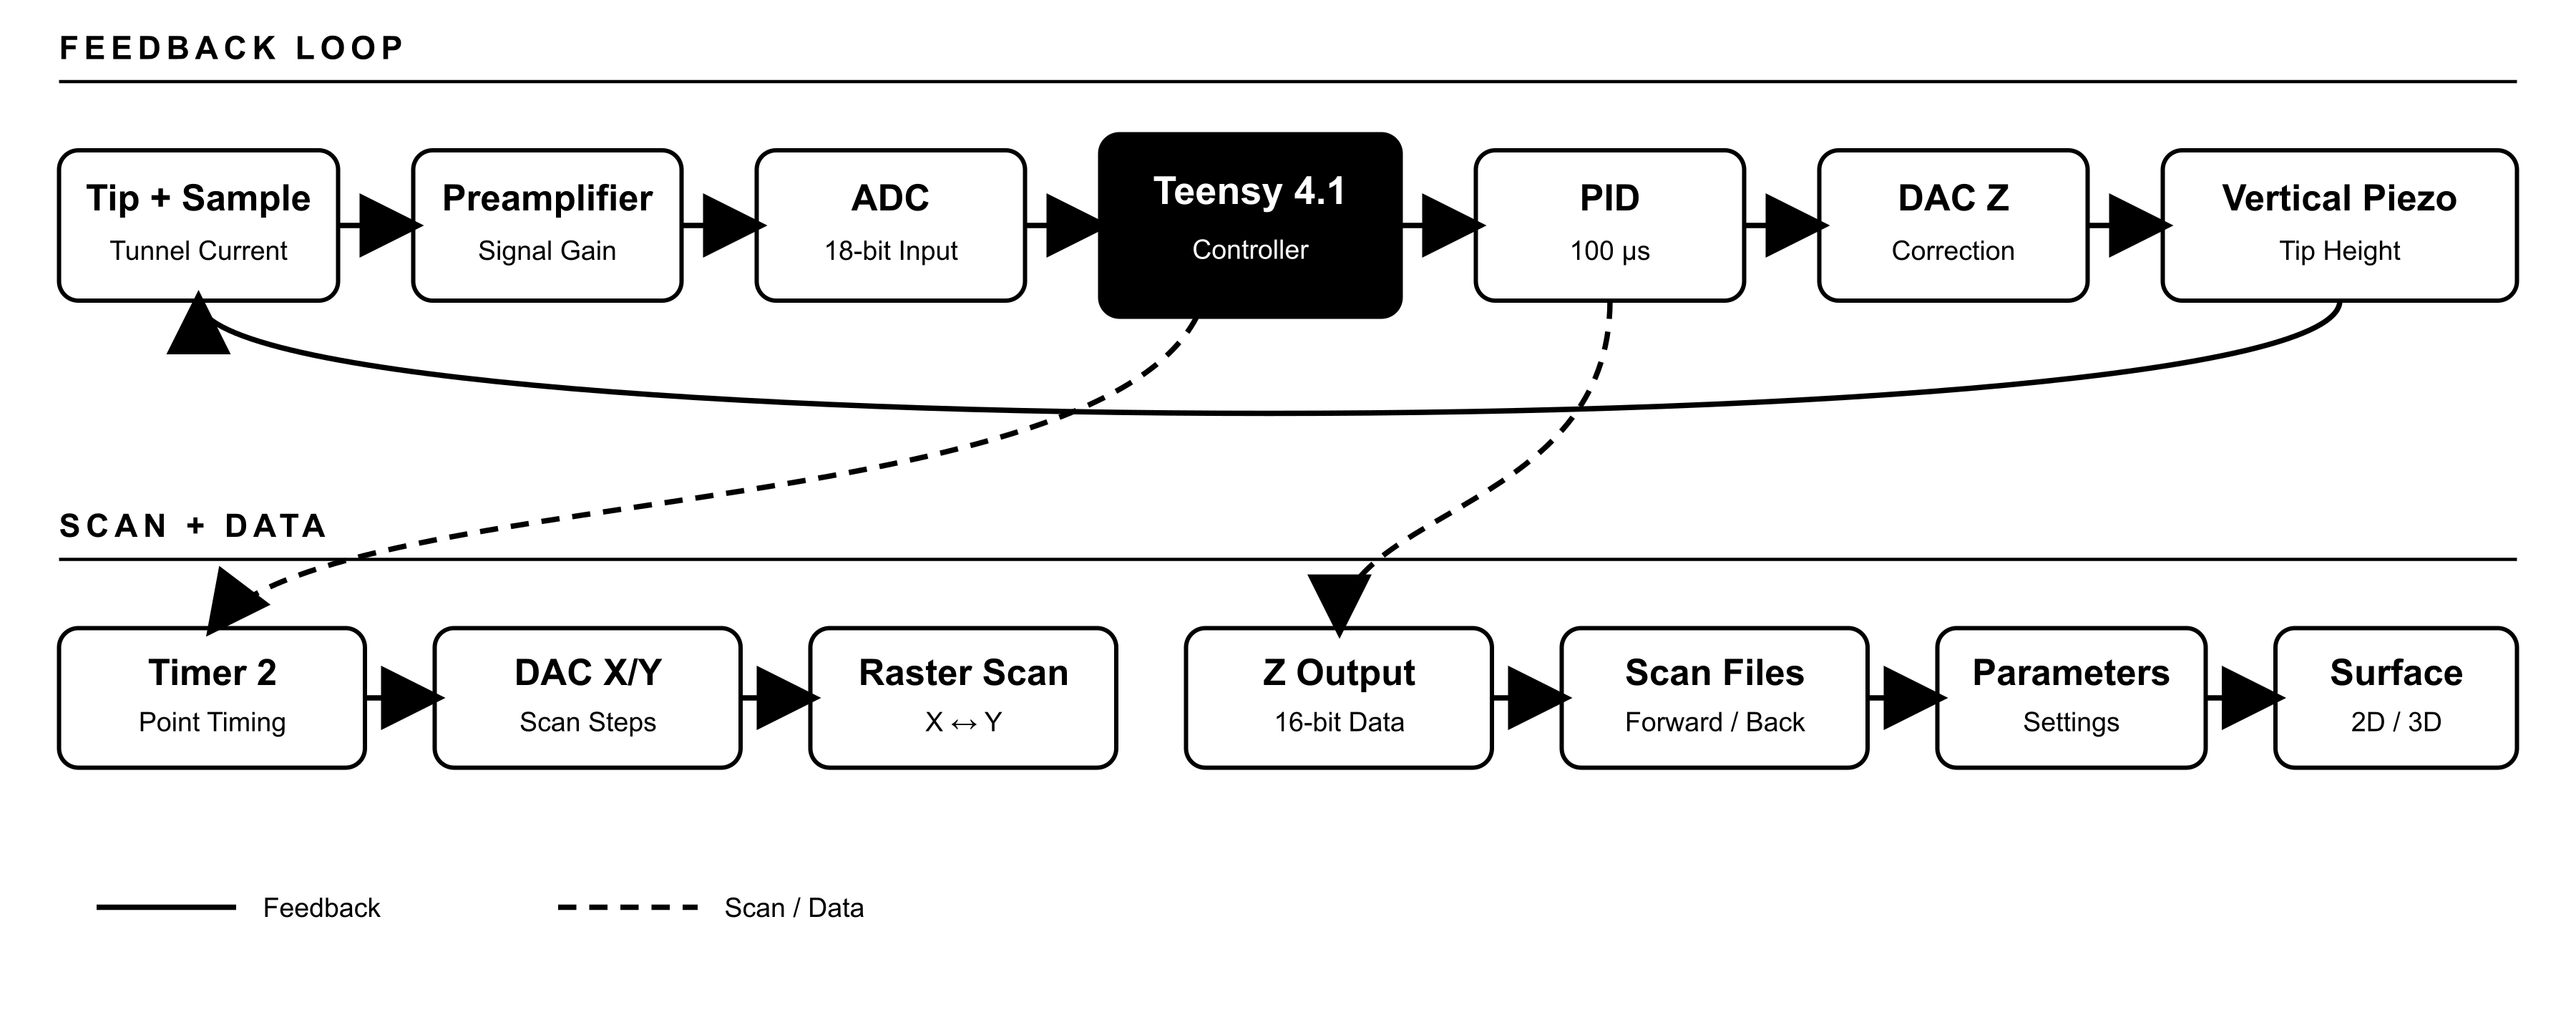
\includegraphics[width=0.96\linewidth]{software-control-flow-large.png}
  \captionsetup{font=footnotesize}
  \captionof{figure}{High-level software architecture. Solid arrows show the
  feedback loop; dashed arrows show scan commands or stored
  data.\textsuperscript{[2,3]}}

  \vspace{4pt}

  % This table is the quick version for people who do not want to follow every
  % arrow in the diagram.
  \begin{tabular}{>{\raggedright\arraybackslash}p{0.29\linewidth}
                  >{\raggedright\arraybackslash}p{0.61\linewidth}}
    \toprule
    Software layer & Primary responsibility \\
    \midrule
    Main program & Initialization, commands, and state selection \\
    Timer 1 & Current measurement and vertical feedback \\
    Timer 2 & Raster coordinates and point storage \\
    File system & Forward, backward, and parameter files \\
    \bottomrule
  \end{tabular}
\end{minipage}

\end{spacing}

\clearpage

% -------------------------------------------------
% CENTER ROW 2, HARDWARE COLUMN
% SHEET 6 OF 12 -- STM OPERATING PRINCIPLES AND PROCEDURE
% -------------------------------------------------
\section{STM Operating Principles and Procedure}

% Explain the physical process from approach to imaging here.
% Keep the detailed code setup on Sheet 5.
% Insert a simple tip/sample drawing here for future if we get too much blank
% space. It should show coarse motion, piezo motion, and the tunneling gap.

\subsection{Quantum-Tunneling Signal}

% Add why the current changes so much with tip--sample distance and why we
% need a conductive sample and a sharp metal tip.

\subsection{Coarse and Fine Positioning}

% Add how the coarse motor, z piezo, and x-y movement each work.

\subsection{Constant-Current Imaging}

% Add how keeping the current steady lets the z correction represent the
% relative surface height.

\subsection{Measurement Procedure}

% Put the final steps here: initialize, set bias/current, approach, turn on
% feedback, set up the scan, collect the data, and pull the tip back.

\clearpage

% -------------------------------------------------
% CENTER ROW 2, SOFTWARE COLUMN
% SHEET 7 OF 12 -- STM CONTROL LOGIC AND SCAN EXECUTION
% -------------------------------------------------
\section{STM Control Logic and Scan Execution}

% This page is about what the code does step by step, not how every file and
% function is arranged. Sheet 5 already handles the overall organization.
\begin{spacing}{1.0}
\small

The firmware converts an STM measurement into a repeatable operating sequence:
approach the sample, confirm a tunneling signal, activate constant-current
feedback, execute the raster scan, and close the data files safely. The
approach, feedback, and scan routines use separate state flags and timer
interrupts so that each process runs only when its required conditions have
been satisfied.\textsuperscript{[2,3]}

\vspace{4pt}

\noindent
\begin{minipage}[t]{0.48\linewidth}
  \vspace{0pt}

  \subsubsection{Automated Approach and Signal Confirmation}

  Feedback is disabled during approach. The program gradually changes the
  vertical DAC output and reads the ADC after each change. When the signal
  exceeds the programmed positive or negative threshold, the ADC is read a
  second time. Only two consecutive threshold crossings are accepted as a
  tunneling signal. If no signal is confirmed during the fine sweep, the
  vertical output retracts, the coarse motor advances one step, and the
  routine can try again.\textsuperscript{[2]}

  \subsubsection{Timer 1: Constant-Current Feedback}

  % This is simplified PID math so visitors can understand the idea without
  % reading the full library. Insert our final Kp, Ki, and Kd here for future.
  After confirmation, Timer~1 executes every \(100\,\mu\mathrm{s}\). It reads
  the ADC, calculates a new PID output, and writes that value to DAC
  channel~0.\textsuperscript{[2]} The supplied PID routine uses
  \[
    u_n=K_Pe_n+I_n-K_D(x_n-x_{n-1}),
  \]
  where \(e_n\) is the setpoint error and \(x_n-x_{n-1}\) is the recent change
  in measured input. The accumulated integral term and final output are
  clamped to the configured limits to prevent requests outside the DAC
  range.\textsuperscript{[3]}

  \subsubsection{Timer 2: Raster-Scan Execution}

  Timer~2 advances \(x\) by one DAC step and stores the current feedback
  output at each point. After the forward line reaches the selected number of
  points, the direction reverses and a backward line is collected. Completing
  both passes resets \(x\), increments \(y\), and starts the next line. When
  the selected number of lines is reached, the timer stops, parameters are
  written, and all files are closed.\textsuperscript{[2]}
\end{minipage}
\hfill
\begin{minipage}[t]{0.49\linewidth}
  \vspace{0pt}
  \centering
  % Keep this diagram simple because the pseudocode right below it gives the
  % extra detail. Update both if the retry path or timer order changes.
  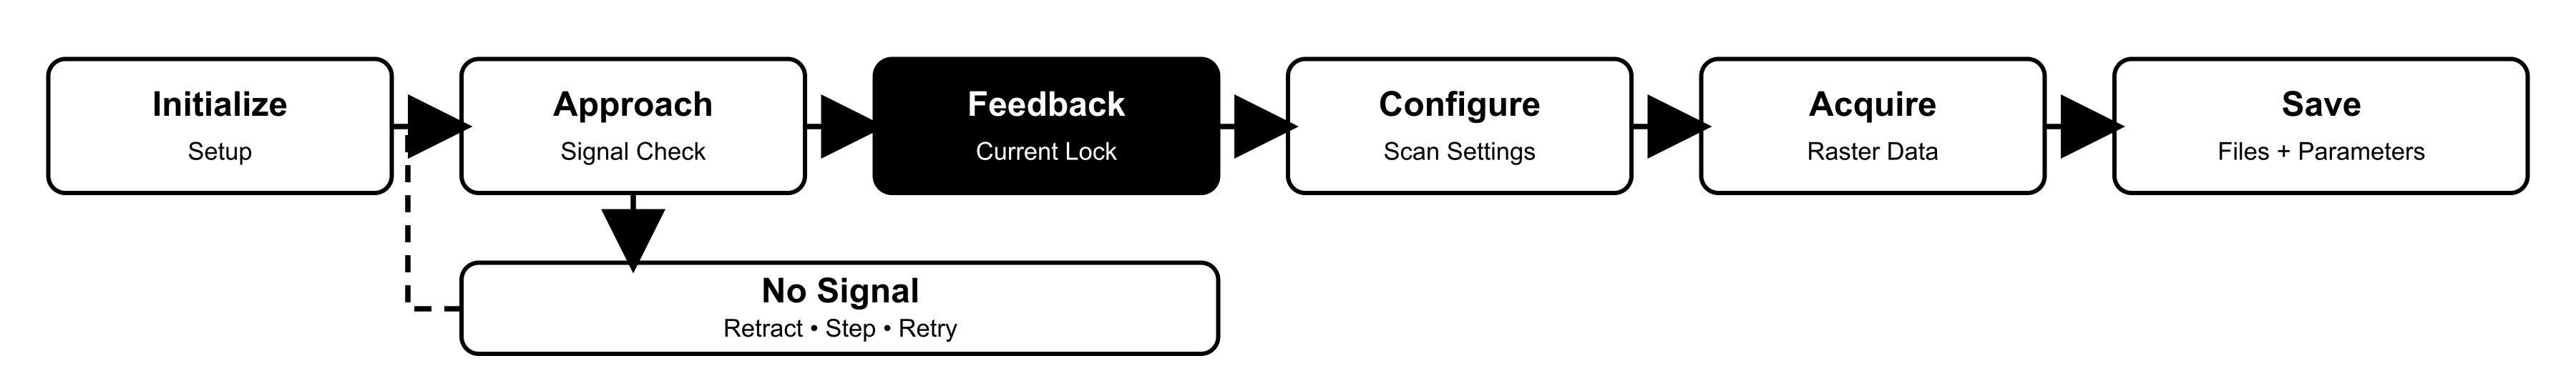
\includegraphics[width=\linewidth]{software-state-sequence.png}
  \captionsetup{font=footnotesize}
  \captionof{figure}{Operating states and the no-signal retry
  path.\textsuperscript{[2]}}

  \raggedright
  \subsubsection{Operating Sequence in Pseudocode}

  % This is not copied code. It is just the logic rewritten so people can read
  % it quickly. Insert any final shutdown or error-handling step here for future.
  The pseudocode emphasizes the conditions that move the controller from one
  operating state to the next.

  \begin{lstlisting}[language={},basicstyle=\ttfamily\scriptsize]
START
  initialize interfaces and safe outputs
  wait for a command
APPROACH
  disable feedback
  sweep Z; read current
  if threshold confirmed twice
    start Timer 1
  else
    retract Z; motor step; retry
FEEDBACK TIMER -- every 100 us
  current <- ADC
  correction <- PID(setpoint - current)
  Z DAC <- limited correction
SCAN TIMER -- each data point
  step X; store correction
  end forward line -> reverse X
  end backward line -> reset X; step Y
  final line -> save parameters; close files
  \end{lstlisting}

  \subsubsection{Why Two Timers?}

  The feedback update must remain fast and regular because tunneling current
  is sensitive to probe height. Scan movement and file writing occur on the
  slower, user-selected acquisition schedule. Separating these schedules
  prevents lateral scanning from determining the feedback update
  rate.\textsuperscript{[2]}
\end{minipage}

\end{spacing}

\clearpage

% -------------------------------------------------
% CENTER ROW 3, HARDWARE COLUMN
% SHEET 8 OF 12 -- SUBSYSTEM TESTING AND CALIBRATION
% -------------------------------------------------
\section{Subsystem Testing and Calibration}

% Put how we tested each part before connecting everything together here.
% Insert a small results table here for future with test value, expected value,
% difference, and whether the part passed.

\subsection{Power-Rail Verification}

% Insert the actual multimeter readings and a board photo here for future.
The positive and negative rails were measured relative to ground with a
multimeter. The trimmer potentiometers were adjusted until the outputs were
\(+15\) V and \(-15\) V.

\subsection{Analog Signal-Chain Verification}

% Insert the oscilloscope screenshots and their input/output settings here for
% future. Make sure the axes and volts-per-division can be read.
The amplifier electronics were driven with a function generator and observed
on an oscilloscope. Input, individual axis, and combined-operation channels
were compared. Summing stages produced the expected combined amplitudes,
while subtraction of matched signals produced an output near zero.

\subsection{ADC Characterization}

% Insert the applied voltage, ADC counts, converted voltage, and percent
% difference here for future. A short calibration graph would work well too.
The ADC was connected to the dual-rail supply and a variable test voltage.
The Teensy 4.1 read the converted value through the Arduino development
environment. The calculated voltage was compared with the applied voltage to
confirm the conversion stage.

\subsection{DAC Characterization}

% Insert the requested DAC value and measured waveform here for future.
The Teensy commanded the DAC to generate a test waveform. The output was
observed on an oscilloscope to verify that the digital commands produced the
expected analog signal.

\clearpage

% -------------------------------------------------
% CENTER ROW 3, SOFTWARE COLUMN
% SHEET 9 OF 12 -- DATA OUTPUT AND SURFACE RECONSTRUCTION
% -------------------------------------------------
\section{Data Output and Surface Reconstruction}

% Write this page like the reader is following the finished workflow. Leave the
% real file names, settings, and results blank until we actually have them.
\begin{spacing}{1.0}
\footnotesize

The controller produces a sequence of vertical feedback corrections as the tip
moves across the sample. The reconstruction program reads the forward scan,
backward scan, and parameter files; verifies their dimensions; reshapes the
values into an \(x,y\) matrix; and converts the result into a surface map.

\vspace{5pt}

\noindent
{\centering
  % This is the overview image. If our real code skips or adds a processing
  % step, update the PNG so the picture still matches the paragraphs.
  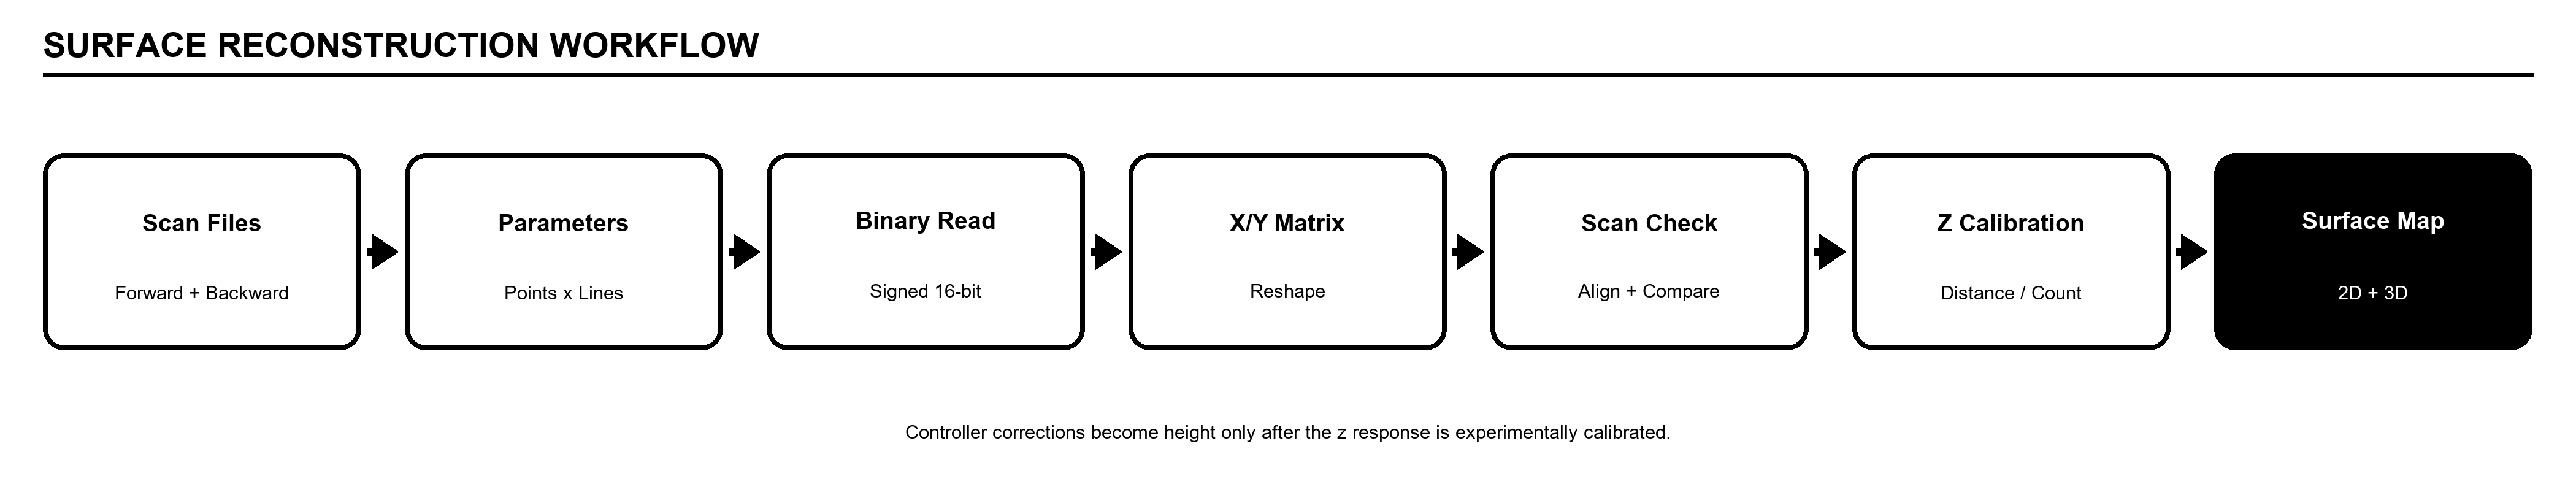
\includegraphics[width=0.90\linewidth]{data-output-surface-reconstruction.png}
  \captionsetup{font=footnotesize}
  \captionof{figure}{Processing workflow from the firmware-defined scan files
  to a reconstructed surface map.\textsuperscript{[2]}}
  \par
}

\vspace{4pt}

\noindent
\begin{minipage}[t]{0.47\linewidth}
  \vspace{0pt}

  \subsubsection{Interpreting the Data Output}

  In constant-current operation, the feedback loop continually changes the
  vertical control signal to keep tunneling current near its setpoint. The
  firmware stores this PID correction as a signed 16-bit value and writes the
  forward and backward passes to separate files.\textsuperscript{[2]} These
  numbers are controller corrections rather than photographs or automatically
  calibrated surface heights.

  The reconstruction program also reads the parameter file, which records the
  requested number of points \(N_x\), number of lines \(N_y\), bias, and
  current setting.\textsuperscript{[2]} It checks that each scan contains
  \(N_xN_y\) stored values before beginning reconstruction. A different file
  length is identified as an incomplete or inconsistent scan rather than being
  silently filled.

  \subsubsection{From a Sequence to a Surface}

  % This formula only explains how a flat file becomes rows and columns.
  % Insert the actual Nx and Ny in the table on the right, not in this formula.
  If \(q_k\) is the \(k\)-th stored correction, the program arranges the
  one-dimensional sequence into a two-dimensional matrix:
  \[
    Q_{j,i}=q_{jN_x+i},
    \qquad
    0\leq i<N_x,\quad 0\leq j<N_y .
  \]
  Each matrix column represents an \(x\)-position and each row represents a
  scan line. The program reverses backward lines into the same spatial
  orientation as the forward lines before making a point-by-point comparison.
\end{minipage}
\hfill
\begin{minipage}[t]{0.50\linewidth}
  \vspace{0pt}

  \subsubsection{Calibration, Comparison, and Visualization}

  % Alpha stays symbolic until we measure it. Do not put nm/count here just
  % because it looks right; insert the measured value in the table later.
  Before calibration, \(Q\) is plotted as relative vertical correction in DAC
  or PID counts. A measured vertical-piezo calibration factor \(\alpha\),
  expressed in distance per count, converts the relative values into height:
  \[
    z_{j,i}=\alpha\left(Q_{j,i}-Q_{\mathrm{ref}}\right).
  \]
  The reference \(Q_{\mathrm{ref}}\) sets the displayed zero level without
  changing the measured height differences. The script displays the forward
  and backward maps separately before combining them because disagreement can
  reveal drift, feedback lag, vibration, or an incorrect line orientation.

  % Insert the final Matplotlib settings here for future, especially any
  % leveling, filtering, interpolation, or color limits that change the image.
  The 2D reconstruction assigns position to the horizontal axes and relative
  correction or calibrated height to color. The 3D view uses the same matrix
  as its vertical coordinate. The program retains the unprocessed matrix before
  applying plane subtraction, line leveling, or filtering, allowing processed
  features to be checked against the original values.

  \subsubsection{Scan and Reconstruction Record}

  % DATA TABLE:
  % Fill this in once we have a complete scan and the code is working.
  % Make sure every physical value has its units.
  \begin{center}
  \renewcommand{\arraystretch}{1.18}
  \begin{tabular}{@{}p{0.46\linewidth}p{0.47\linewidth}@{}}
    \toprule
    \textbf{Record} & \textbf{Value} \\
    \midrule
    Forward-scan file & \rule{0.92\linewidth}{0.4pt} \\
    Backward-scan file & \rule{0.92\linewidth}{0.4pt} \\
    Parameter file & \rule{0.92\linewidth}{0.4pt} \\
    Matrix size, \(N_x\times N_y\) & \rule{0.92\linewidth}{0.4pt} \\
    Bias and current setpoint & \rule{0.92\linewidth}{0.4pt} \\
    Vertical calibration, \(\alpha\) & \rule{0.92\linewidth}{0.4pt} \\
    Processing code/version & \rule{0.92\linewidth}{0.4pt} \\
    \bottomrule
  \end{tabular}
  \end{center}

  % Once we have the data, replace this with how we ran the scan, whether it
  % finished, and anything weird that happened while collecting it.
  \textit{Add about the collected data and scan conditions.}

  % Once the code works, replace this with what it checks, what processing we
  % used, and where the script is in clustered.
  \textit{Add about the reconstruction code and processing choices.}

  % Once we have the final maps, replace this with how the forward and backward
  % scans compare and what we can actually see in the surface.
  \textit{Add about the reconstructed surface and scan agreement.}
\end{minipage}

\end{spacing}

\end{landscape}

% =================================================
% RIGHT PANEL: THREE PORTRAIT SHEETS
% =================================================

% -------------------------------------------------
% SHEET 10 OF 12 -- RESULTS AND UNCERTAINTY ANALYSIS
% -------------------------------------------------
\section{Results and Uncertainty Analysis}

% Put the main results here, along with the limits we can actually support.
% Insert the final headline result here for future. This should be the one or
% two things we would tell someone if they only read this page.

\subsection{Key Findings}

% Only add results that our final tests and data actually show.
% Insert a small table or figure here for future if numbers explain the result
% better than another paragraph.

\subsection{Sources of Uncertainty}

% Things to check: vibration, electrical noise, thermal drift, piezo
% hysteresis/creep, tip shape, calibration, feedback tuning, and scan speed.
% For the final version, say which of these we actually observed instead of
% listing every possible STM problem.

\subsection{Recommended Improvements}

% For each improvement, say which problem we actually saw that it would fix.
% Insert the highest-priority fix first for future, then explain what measurement
% would show that the fix worked.

\clearpage

% -------------------------------------------------
% SHEET 11 OF 12 -- SUPPLEMENTARY FIGURES
% -------------------------------------------------
\section{Supplementary Figures}

% Put any extra graphs that do not fit on Sheet 9 here.
% Every graph still needs labeled axes, units, a caption, and a quick
% explanation of what it shows.

% Add the extra graphs and number comparisons here.
% Insert figure 1 here for future.
% Insert figure 2 here for future if it adds something different.
% If we only have one useful extra graph, leave the rest of the page open
% instead of stretching it or adding filler.

\clearpage

% -------------------------------------------------
% SHEET 12 OF 12 -- REFERENCES AND ACKNOWLEDGMENTS
% -------------------------------------------------
\section{References and Acknowledgments}

% If we add a new source anywhere else, add it here and make sure the little
% citation number in the text matches this list.
\noindent
\begin{minipage}[t]{0.72\textwidth}
  \vspace{0pt}
  \subsection{References}

  \begin{enumerate}
    \item S. Chiang, ``Additional Quantum Mechanics Discussion,''
    \textit{QMnotes1.pdf}, COSMOS course handout, 2026.

    \item S. Chiang, \textit{Teensy STM11A}, STM controller source code,
    University of California, Davis, 2025.

    \item B. Beauregard, \textit{Arduino PID Library}, version 1.1.1,
    timer-interrupt modification by S. Chiang, course software archive.

    \item souuk, \textit{clustered: STM Project Files and Citation-Source
    Paths}, GitHub repository, 2026. Available:
    \href{https://github.com/souuk/clustered}{github.com/souuk/clustered}.
    Source locations within the supplied course archive are listed in the
    repository's
    \href{https://github.com/souuk/clustered\#citation-path-index}
    {citation path index}.
  \end{enumerate}
\end{minipage}
\hfill
\begin{minipage}[t]{0.23\textwidth}
  \vspace{0pt}
  \raggedleft
  % This makes the QR code straight from the link, so we do not need to upload
  % another PNG for it in Overleaf.
  \href{https://github.com/souuk/clustered}{%
    \qrcode[height=1.25in]{https://github.com/souuk/clustered}%
  }

  \vspace{5pt}
  {\small\bfseries STM source code\par}
  {\footnotesize github.com/souuk/clustered\par}
\end{minipage}

\subsection{Acknowledgments}

% Insert any other instructors, mentors, or group-specific help here for future.
We thank Professor Shirley Chiang for providing the spring-suspension
platform, quantum-mechanics notes, STM controller program, and other course
materials used in this project.

\end{document}
